% 原书 p.187–p.194（PDF p.195–p.202）

% >>> p195
\section{形状不变量（Shape Invariant）}

\begin{keytakeaways}
\begin{itemize}
  \item 几何图像：拉格朗日子流形 $L$ 携带两个基本量——刘维尔类 $[\lambda_L]$（记录
        被 $L$ 围出的辛面积）与 Maslov 指标 $\mu$（记录沿 $L$ 的 Lagrangian 平面
        的旋转）。两者合起来，可以在 $\R^4$ 的拉格朗日环面上典范地选出一组有序基。
  \item 核心工具：长正合列与 (7.16) 的「面积 = 积分」解释；Robbin--Salamon 指标的
        一半（定义 7.3.1）；命题 7.3.1 给出的存在唯一性。
  \item 关键定理：形状不变量 $\mathrm{Sh}^+(X)$（定义 7.3.2）在辛嵌入下单调
        （练习 7.3.1），从而是一种「二维/非线性」的辛容量；定理 7.3.1 给出
        $Z^4(R)$、$B^4(R)$、$P(a,b)$、$E(a,b)$ 的显式形状不变量。
  \item 本节结论：例 7.3.4 用形状不变量排除 $P(1,2)$ 到 $E(1.5,3)$ 的辛嵌入，
        而体积比较与 Gromov 宽度都无能为力——这正是「非线性」容量的价值所在。
\end{itemize}
\end{keytakeaways}

给定星形区域 $X\subset(\C^2,\dd\lambda_{\mathrm{std}})
=(\R^4,\dd\lambda_{\mathrm{std}})$，除了 6.4 节引入的各种辛容量（它们是 $\R$
中的标量序列）之外，近期还发展出「非线性」容量，其灵感来自 Sikorav
[208,209] 与 Eliashberg [75] 的先驱工作。

% [Tutor Note: 原文疑误——本段原文将 Sikorav 拼作 "J. C. Sikarov"（正确拼写为
% Jean-Claude Sikorav，缩写 J.-C. Sikorav），属于人名笔误。译文保留书名号内的
% 文献编号 [208,209]，正文改用通行拼写 Sikorav，并已记入审校记录。]

任何这样的区域 $X$ 都可视为带边界的恰当辛流形 $(X,\dd\lambda_{\mathrm{std}})$。
设 $L\subset(X,\dd\lambda_{\mathrm{std}})$ 是嵌入的拉格朗日子流形。注意
$\lambda_L:=\lambda_{\mathrm{std}}|_L$ 满足
\begin{equation}\tag{7.15}
  \dd\lambda_L=\dd(i^*\lambda_{\mathrm{std}})=i^*\dd\lambda_{\mathrm{std}}=0,
\end{equation}
其中 $i\colon L\hookrightarrow X$ 是包含映射。换言之，$\lambda_L$ 是
$\Omega^1(L)$ 中的闭 1-形式，这意味着 $[\lambda_L]$ 代表 $H^1(L;\R)$ 中的一个
上同调类，称为 $L$ 在 $(X,\dd\lambda_{\mathrm{std}})$ 中的\textbf{刘维尔类}
（Liouville class）。

% >>> p196
为了更具体地描述类 $[\lambda_L]$，让我们在 $H_1(L;\R)$ 的类上对它赋值。这里，
包含映射 $i\colon L\to W$ 诱导出如下长正合列
\[
  \cdots\to H_2(L;\Z)\to H_2(X;\Z)\to H_2(X,L;\Z)
  \to H_1(L;\Z)\to H_1(X;\Z)\to\cdots.
\]
由于 $H_{*\ge1}(X;\Z)=0$（$X$ 可缩），有 $H_2(X,L;\Z)\cong H_1(L;\Z)$。于是
$H_2(X,L;\R)\cong H_1(L;\R)$。这意味着对任何类 $a=[\alpha]\in H_1(L;\R)$，
存在 2-链 $\Sigma\subset X$ 使得 $\partial\Sigma=\alpha$。因此，
\begin{equation}\tag{7.16}
  [\lambda_L](a)=\int_a\lambda_L
  =\int_{\partial\Sigma}\lambda_L=\int_\Sigma\dd\lambda_{\mathrm{std}},
\end{equation}
其中最后一步意味着：$[\lambda_L]$ 实际上度量了界定闭链 $\alpha$ 的（任意）
2-链 $\Sigma$ 的辛面积。注意，若在 $X$ 中取 2-链 $\Sigma_1$ 与 $\Sigma_2$ 使得
$\partial\Sigma_1=\partial\Sigma_2=\alpha$，则
\[
  \int_{\partial\Sigma_1}\lambda_L-\int_{\partial\Sigma_2}\lambda_L
  =\int_{\partial(\Sigma_1\#\overline{\Sigma}_2)}\lambda_L
  =\int_{\Sigma_1\#\overline{\Sigma}_2}\dd\lambda_{\mathrm{std}}=0,
\]
其中最后一步来自 $H_2(X;\R)=0$。所以赋值 $[\lambda_L](a)$ 是良定义的。

% [Tutor Note: 原文疑误——本段原文 "the inclusion $i\colon L\to W$ induces the
% following long exact sequence" 中的 $W$ 应为 $X$：全段其余部分（以及长正合列
% 本身）都使用 $X$，且 (7.16) 的积分区域也在 $X$ 中。译文按 $X$ 处理，并已记入
% 审校记录。另请注意：长正合列这一步用到了 $H_{*\ge1}(X;\Z)=0$ 与 $H_2(X;\R)=0$
% 两个事实，后者保证 $[\lambda_L](a)$ 与 $\Sigma$ 的选取无关。]

\begin{wexam}{7.3.1}
  设 $L\subset(\R^4,\dd\lambda_{\mathrm{std}})$ 是嵌入的拉格朗日 2-环面
  （参看 (1.14)）。为描述 $[\lambda_L]\in H^1(L;\R)=H^1(\T^2;\R)$，固定标准基
  $e_1,e_2\in H_1(L;\Z)=H_1(\T^2;\Z)$，即 $e_1$ 由沿经圈（longitude）方向只
  绕行一次的 1-闭链代表，$e_2$ 由沿子午圈（meridian）方向只绕行一次的 1-闭链
  代表。则 $[\lambda_L]$ 的
  赋值给出一个数对 $(r,s)\in\R^2$，它度量了界定 $e_1$ 与 $e_2$ 的圆盘的辛面积。
  见图 7.11。作为更具体的例子，考虑分裂 2-环面
  $S^1(r)\times S^1(s)\subset(\R^4,\dd\lambda_{\mathrm{std}})$，其中 $S^1(r)$
  与 $S^1(s)$ 的半径分别为 $\sqrt{r/\pi}$ 与 $\sqrt{s/\pi}$。则
  \[
    [\lambda_L](e_1)=\int_{\Sigma_1}\dd\lambda_{\mathrm{std}}=r
    \quad\text{且}\quad
    [\lambda_L](e_2)=\int_{\Sigma_2}\dd\lambda_{\mathrm{std}}=s,
  \]
  其中 $\Sigma_1$ 与 $\Sigma_2$ 分别是 $\R^2$ 中面积为 $r$ 与 $s$ 的标准
  2-圆盘。\hfill$//$
\end{wexam}

\begin{figure}[htbp]
  \centering
  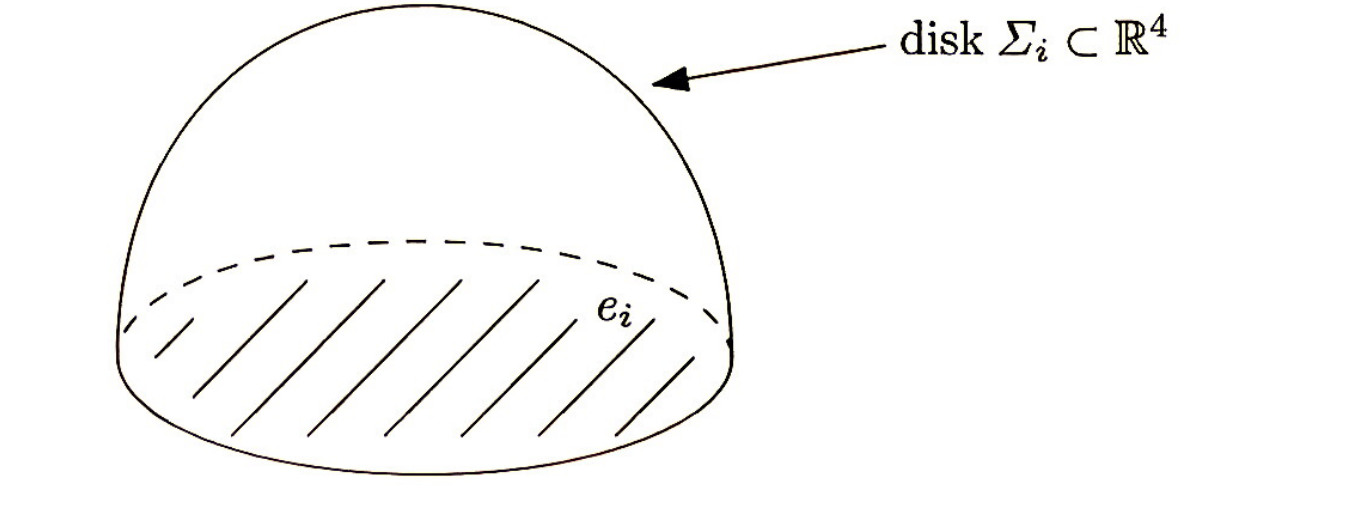
\includegraphics[width=0.58\linewidth]{figures/fig_p196_1.png}
  \caption*{图 7.11\quad 以 $e_i$ 为边界的圆盘
    $\Sigma_i\subset\R^4$（原书 p.188, Figure 7.11；PDF p.196）}
\end{figure}

% >>> p197
注意，当 $L\subset(X,\dd\lambda_{\mathrm{std}})$ 是嵌入的拉格朗日环面时，上面
例 7.3.1 所说明的 $[\lambda_L]\colon H_1(L;\R)\to\R$ 只有在固定了
$H_1(L;\R)$ 的一组有序基 $(e_1,e_2)$ 之后才有意义。$(\R^4,
\dd\lambda_{\mathrm{std}})$ 上的一个微分同胚很容易改变这组基 $(e_1,e_2)$，
从而得到的数对 $(r,s)\in\R^2$ 也会随之改变。见图 7.12。

\begin{figure}[htbp]
  \centering
  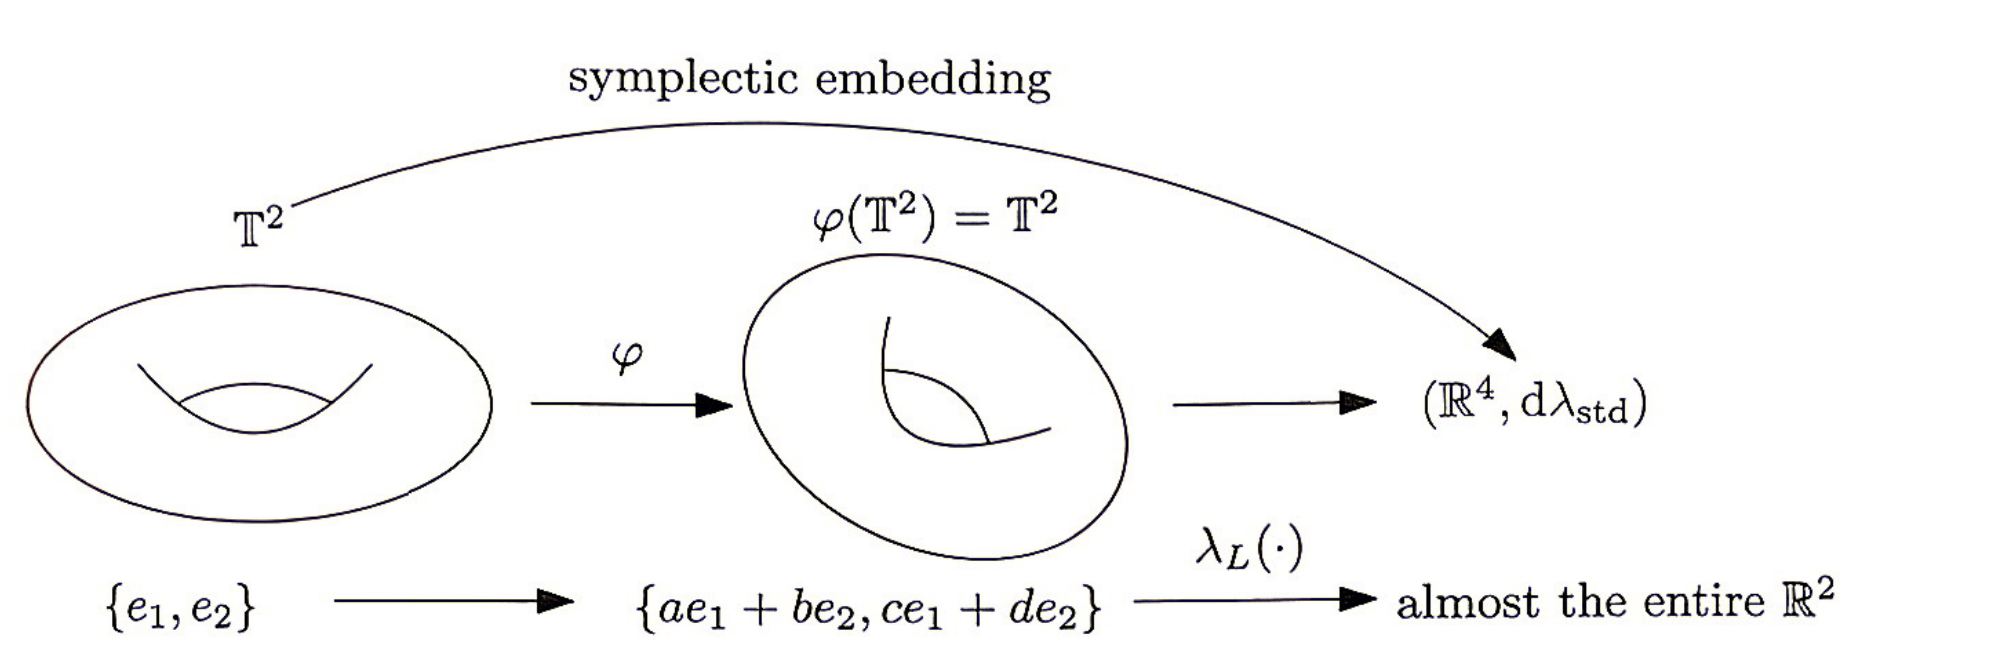
\includegraphics[width=0.9\linewidth]{figures/fig_p197_1.png}
  \caption*{图 7.12\quad 在 $\varphi\in\Diff(\T^2)$ 下有序基
    $(e_1,e_2)$ 的改变（原书 p.189, Figure 7.12；PDF p.197）}
\end{figure}

\begin{wexam}{7.3.2}
  考虑环面区域 $X_\Omega\subset\R^4$。对 $(r,s)=(1,2)$，很难分辨
  $L=S^1(1)\times S^1(2)$ 还是 $L=\varphi(S^1(1)\times S^1(1))$，其中 $\varphi$
  是 $(X,\dd\lambda_{\mathrm{std}})$ 上某个微分同胚（辛同胚），其诱导映射
  $\varphi_*$ 在 $H_1(L;\R)$ 上把 $(e_1,e_2)$ 送到 $(e_1,e_1+e_2)$。
  \hfill$//$
\end{wexam}

为解决这一问题，我们需要引入另一个量，使有序基能以某种典范的方式固定下来。
这引出下述概念，它其实植根于 5.5 节。

\begin{wdefn}{7.3.1（Maslov 指标）}
  给定 $(\R^4,\dd\lambda_{\mathrm{std}})$ 中嵌入的拉格朗日环面 $L$，对任何类
  $\gamma_*([S^1])\in H_1(L;\Z)$（其中 $\gamma\colon S^1\to L$），如下关联一个
  数 $\mu(e)$，它是 Robbin--Salamon 指标（见 (5.27)）的\emph{一半}，其输入为：
  \begin{enumerate}[label=(\roman*)]
    \item 拉回丛 $\gamma^*TL$ 定义了 $S^1$ 上秩为 $2$ 的向量丛，其纤维是 $TM$
          中的拉格朗日 2-平面。
    \item 固定 $T_{\gamma(0)}L$ 的一组基，则当沿底空间 $S^1$ 移动时，它给出
          $\mathrm{Sp}(2)$ 中辛矩阵构成的环路
          $A:=\{A(t)\}_{t\in[0,1]}$。
    \item （回忆我们定义了对称矩阵
          $S(t)=-\Omega\dot A(t)A(t)^{-1}$。）这里，我们把它限制到
          $T_{\gamma(t)}L$，即 $S(t)|_{T_{\gamma(t)}L}$，并把 (5.26) 中相应的
          交叉形式记作 $\Gamma^{\mathrm{Lag}}(A,t)$。
  \end{enumerate}
  该映射 $\mu\colon H_1(L;\Z)\to\Z$ 称为类 $e\in H_1(L;\Z)$ 的
  \textbf{Maslov 指标}。
\end{wdefn}

% [Tutor Note: 含糊点拨——定义 7.3.1 中「取 Robbin--Salamon 指标的一半」是本节
% 最容易含糊的一步：一般闭道路的 Robbin--Salamon 指标是整数，而拉格朗日环面上
% 由 $\gamma_*([S^1])$ 给出的环路其指标恒为偶数，故取半得到整数 $\mu(e)$；这也
% 解释了例 7.3.3 中 $\mu(e)=2$ 而非 $4$。核对要点：(i) $S(t)$ 的对称性来自
% $\Omega\dot A A^{-1}$ 的对称性，而 $-\Omega\dot A A^{-1}$ 只在限制到
% Lagrangian 平面 $T_{\gamma(t)}L$ 后才成为对称双线性形式；(ii) 交叉形式的
% 符号约定必须与 (5.26) 一致，否则 $\mu$ 整体差一个符号。]

\begin{wrem}{7.3.1}
  (i) 注意定义 7.3.1 中的条件 (iii) 只考虑双线性形式 $\Gamma(A,t)$ 的「一半」。
  又因为辛矩阵的道路 $A$ 是一个环路，如例 5.5.6 所讨论，$\mu$ 的取值落在 $\Z$
  中。(ii) 可以验证 $\mu(e)$ 与代表元 $\gamma\colon S^1\to L$ 的选取无关。
  (iii) $\mu\colon H_1(L;\Z)\to\Z$ 是同态。
\end{wrem}

% >>> p198
下述例子（与定义 7.3.1 相比维数降低了）是例 5.5.7 的相对版本。

\begin{wexam}{7.3.3}
  考虑拉格朗日子流形 $L=S^1\subset\R^2$（见图 7.13）。取初始点
  $\gamma(0)=(1,0)\in\R^2$（即 $t=0$ 时）。则此时 $\mathrm{Sp}(2)$ 中的辛矩阵
  环路由旋转给出，即
  \[
    A(t)=\begin{pmatrix}\cos(2\pi t)&\sin(2\pi t)\\
    -\sin(2\pi t)&\cos(2\pi t)\end{pmatrix}\in\mathrm{Sp}(2).
  \]
  由定义 7.3.1，我们有
  \[
    \mu(e)=2\cdot\frac12\left(\operatorname{sign}
    \bigl(\Gamma^{\mathrm{Lag}}(A,0)\bigr)
    +\sum_{t\in(0,1)}\operatorname{sign}
    \bigl(\Gamma^{\mathrm{Lag}}(A,t)\bigr)\right)
    =2\cdot\frac12\cdot2=2.
  \]
  换言之，$\R^2$ 中一次完整旋转的 Maslov 指标为 $2$。\hfill$//$
\end{wexam}

\begin{figure}[htbp]
  \centering
  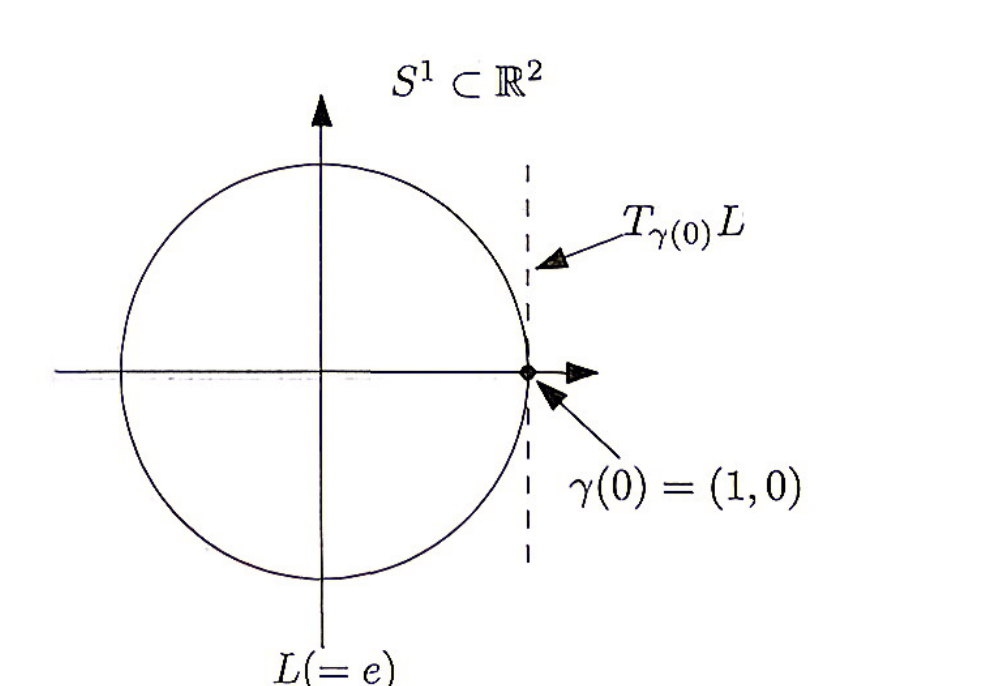
\includegraphics[width=0.52\linewidth]{figures/fig_p198_1.png}
  \caption*{图 7.13\quad $\R^2$ 中的一维拉格朗日环面（原书 p.190,
    Figure 7.13；PDF p.198）}
\end{figure}

与 $[\lambda_L]$ 的作用类似，当 $H_1(L;\Z)$ 的基在微分同胚
$\varphi\in\Diff(L)=\Diff(\T^2)$ 下改变时，$\mu(e)$ 的值也可能相应地改变。

以一种颇令人惊讶的方式，若同时施加来自 $[\lambda_L]$ 与 $\mu$ 的两个赋值约束，
则有序基可以被固定下来，如下述命题所示。为简化记号，记 $\Omega(e)$ 为
$e\in H_1(L;\Z)$ 在 $[\lambda_L]$ 下的赋值。

\begin{wprop}{7.3.1（[114] 中的引理 1.1）}
  若 $L\subset\R^4$ 是拉格朗日环面，则存在 $H_1(L;\Z)$ 的有序基 $(e_1,e_2)$，
  满足 $\mu(e_1)=\mu(e_2)$ 且 $0<\Omega(e_1)\le\Omega(e_2)$。特别地，当
  $\Omega(e_1)\ne\Omega(e_2)$ 时，满足 $0<2\Omega(e_1)\le\Omega(e_2)$ 的这样的
  基 $(e_1,e_2)$ 是唯一的。
\end{wprop}

命题 7.3.1 的证明基于下述经典事实。

\whead{事实}{7.3.1（[233] 中的定理 A，或 [178] 中的定理 2.1）}若
$L\hookrightarrow\R^4$ 是拉格朗日环面，则存在 $e\in H_1(L;\Z)$ 使得
$\mu(e)=2$ 且 $\Omega(e)>0$。此外，这样的 $e$ 是本原的，即它不是任何其他类的
迭代。

% [Tutor Note: 含糊点拨——事实 7.3.1 是本节唯一未加证明的深层输入，绝非定义
% 7.3.1 的直接推论：它断言 $\R^4$ 中拉格朗日环面上必存在 Maslov 指标为 2 且
% 面积为正的本原类。其证明需要伪全纯曲线/辛场论（SFT）式的整体工具（可参看
% 本章 9.7 节所述的 neck-stretching 技术），原始出处见 [233] 与 [178]。读者
% 若只从线性代数出发试图「验证」此事实，必定徒劳。]

% >>> p199
\begin{wproof}[命题 7.3.1 的证明]
  由事实 7.3.1，有一个类 $e=e_1$ 满足 $\mu(e_1)=2$。把它扩充为
  $H_1(L;\Z)$ 的有序基 $(e_1,e_2)$。由于 $\mu(e_2)$ 总是偶数，从 $e_2$ 中减去
  适当多个 $e_1$，我们可以假设 $\mu(e_2)=2$。然后按 $\Omega(e_2)$ 的符号分
  情况处理。

  若 $\Omega(e_2)>0$，交换 $e_1,e_2$ 即得所需的一对 $(e_1,e_2)$。若
  $\Omega(e_2)<0$，则把 $e_2$ 换成 $2e_1-e_2$，使得
  \[
    \mu(2e_1-e_2)=2\cdot2-2=2
    \quad\text{且}\quad
    \Omega(2e_1-e_2)=2\Omega(e_1)-\Omega(e_2)>0.
  \]
  因此，我们总可以假设 $\Omega(e_2)\ge\Omega(e_1)>0$。若
  $\Omega(e_1)>\Omega(e_2)$，考虑所有保持 Maslov 类与定向的 $\Z$ 上基变换
  （由 $\T^2$ 上的微分同胚诱导）：
  \[
    \begin{pmatrix}a&b\\c&d\end{pmatrix}\cdot
    \begin{pmatrix}e_1<本地路径>
    =\begin{pmatrix}ae_1+be_2\\ce_1+de_2\end{pmatrix},
  \]
  即 $a+b=1$、$c+d=1$ 且 $ad-bc=1$。这意味着这样的矩阵具有如下形式
  \[
    \begin{pmatrix}a+1&-a\\a&1-a\end{pmatrix}
  \]
  其中 $a\in\Z$。新的面积类为
  \begin{align*}
    \begin{pmatrix}a+1&-a\\a&1-a\end{pmatrix}\cdot
    \begin{pmatrix}\Omega(e_1)\\\Omega(e_2)\end{pmatrix}
    &=\begin{pmatrix}(a+1)\Omega(e_1)-a\Omega(e_2)\\
      a\Omega(e_1)+(1-a)\Omega(e_2)\end{pmatrix}\\
    &=\begin{pmatrix}\Omega(e_1)-a(\Omega(e_2)-\Omega(e_1))\\
      \Omega(e_2)-a(\Omega(e_1)-\Omega(e_2))\end{pmatrix}.
  \end{align*}
  注意到第一个因子为正，恰当
  $a<\dfrac{\Omega(e_1)}{\Omega(e_2)-\Omega(e_1)}$。又注意到
  \[
    \Omega(e_2)-a(\Omega(e_2)-\Omega(e_1))
    \ge2\bigl(\Omega(e_1)-a(\Omega(e_2)-\Omega(e_1))\bigr),
  \]
  它等价于
  \[
    a\ge\frac{\Omega(e_1)}{\Omega(e_2)-\Omega(e_1)}-1.
  \]
  于是存在唯一的 $a\in\Z$ 落在区间
  $\Bigl[\dfrac{\Omega(e_1)}{\Omega(e_2)-\Omega(e_1)}-1,
  \dfrac{\Omega(e_1)}{\Omega(e_2)-\Omega(e_1)}\Bigr)$ 中。因此，所求的有序基为
  $\bigl((a+1)e_1-ae_2,\ ae_1+(1-a)e_2\bigr)$。
\end{wproof}

% [Tutor Note: 原文疑误——上式中第二个分量原文印作
% $\Omega(e_2)-a(\Omega(e_1)-\Omega(e_2))$，与紧接其前的等式
% $a\Omega(e_1)+(1-a)\Omega(e_2)$ 不符；按后者应为
% $\Omega(e_2)-a(\Omega(e_2)-\Omega(e_1))$。只有修正后的形式才能推出原文下一个
% 不等式与 $a\ge\Omega(e_1)/(\Omega(e_2)-\Omega(e_1))-1$ 的结论。译文保留原文
% 写法并已记入审校记录。]

命题 7.3.1 使我们能把上面的对应
$L\stackrel{[\lambda_L]}{\longmapsto}(\Omega(e_1),\Omega(e_2))$ 精化为如下
定义。

\begin{wdefn}{7.3.2（形状不变量）}
  给定星形区域 $X\subset(\R^4,\dd\lambda_{\mathrm{std}})$，定义 $X$ 的
  \textbf{形状不变量}为
  \[
    \mathrm{Sh}^+(X):=\left\{(\Omega(e_1),\Omega(e_2))\in\R^2\ \middle|\
    \begin{array}{l}
      (e_1,e_2)\ \text{是}\ H_1(L;\Z)\ \text{的有序基，}\\
      \text{且满足命题 7.3.1 的条件}
    \end{array}\right\}
  \]
  其中条件遍历 $L$ 取遍 $(X,\dd\lambda_{\mathrm{std}})$ 中所有嵌入的拉格朗日
  环面。
\end{wdefn}

% >>> p200
\begin{wrem}{7.3.2}
  若 $\Omega(e_1)\ne\Omega(e_2)$，则有序基 $(e_1,e_2)$ 的选取没有歧义。若
  $\Omega(e_1)=\Omega(e_2)$，则这样的基 $(e_1,e_2)$ 不唯一。然而可以验证，对
  任何其他满足 $\mu(e'_i)=2$（$i=1,2$）的有序基 $(e'_1,e'_2)$，总有
  $\Omega(e'_1)=\Omega(e'_2)=\Omega(e_1)=\Omega(e_2)$。因此 $\mathrm{Sh}^+(X)$
  是良定义的。
\end{wrem}

下述结果综合了各种定理，说明对一些基本环面区域，相应的形状不变量是什么样子。

\begin{wthm}{7.3.1（[46]；[113] 中的定理 1 与定理 3；[114] 中的定理 1.3）}
  对 $X_\Omega=Z^4(R)$，其形状不变量 $\mathrm{Sh}^+(Z^4(R))$ 为
  \[
    \mathrm{Sh}^+(Z^4(R))
    =\bigl\{(x_1,x_2)\in\R^2_{\ge0}\mid x_2\ge2x_1,\ x_1<R\bigr\}
    \cup\bigl\{x_1=x_2,\ x_2<R\bigr\}.
  \]
  对 $X_\Omega=B^4(R)$，
  \[
    \mathrm{Sh}^+(B^4(R))
    =\left\{(x_1,x_2)\in\R^2_{\ge0}\ \middle|\
    x_2\ge2x_1,\ x_1<\frac{R}{3}\right\}
    \cup\bigl\{x_1=x_2,\ x_2<R\bigr\}.
  \]
  对 $X_\Omega=P(a,b)$（$a\le b$），
  \[
    \mathrm{Sh}^+(P(a,b))
    =\left\{(x_1,x_2)\in\R^2_{\ge0}\ \middle|\
    \begin{array}{l}
      x_1<\dfrac{a}{2},\ x_2>0\\
      \text{或}\\[2pt]
      a>x_1\ge\dfrac{a}{2},\ x_2<b
    \end{array}\right\}
    \cap\left(\begin{array}{c}\{x_2\ge2x_1\}\\ \cup\\ \{x_1=x_2\}\end{array}\right).
  \]
  最后，对 $X_\Omega=E(a,b)$（$\dfrac{b}{a}\in\N_{\ge2}$），
  \[
    \mathrm{Sh}^+(E(a,b))
    =\left\{(x_1,x_2)\in\R^2_{\ge0}\ \middle|\
    \begin{array}{l}
      x_1<\dfrac{a}{2},\ x_2>0\\
      \text{或}\\[2pt]
      x_1\ge\dfrac{a}{2},\ \dfrac{x_1}{a}+\dfrac{x_2}{b}<1
    \end{array}\right\}
    \cap\left(\begin{array}{c}\{x_2\ge2x_1\}\\ \cup\\ \{x_1=x_2\}\end{array}\right).
  \]
\end{wthm}

这些形状不变量正是图 7.14 所描绘的。

定理 7.3.1 的证明颇为复杂。显然它分成两部分。其一，用同调机器导出（定量的）
关于恰当拉格朗日（环面）嵌入存在性的障碍，这给出 $\mathrm{Sh}^+(X_\Omega)$ 的
区域（作为上界）。其二，通过显式构造嵌入的拉格朗日环面，得到
$\mathrm{Sh}^+(X_\Omega)$ 的下界。更具体地说，第一部分可借助伪全纯曲线以及称为
颈部拉伸（neck-stretching）的有力技术来完成。更多细节见 9.7 节。

\begin{wexer}{7.3.1}
  证明：对两个星形区域 $X,Y\subset(\R^4,\dd\lambda_{\mathrm{std}})$，若存在辛
  嵌入 $\varphi\colon X\to Y$，则 $\mathrm{Sh}^+(X)\subset\mathrm{Sh}^+(Y)$。
\end{wexer}

该练习表明，$\mathrm{Sh}^+(\cdot)$ 可以看作一种「二维」辛容量，用来排除
$(\R^4,\dd\lambda_{\mathrm{std}})$ 中星形区域之间的嵌入。下面是一个具体的例子。

% >>> p201
\begin{figure}[htbp]
  \centering
  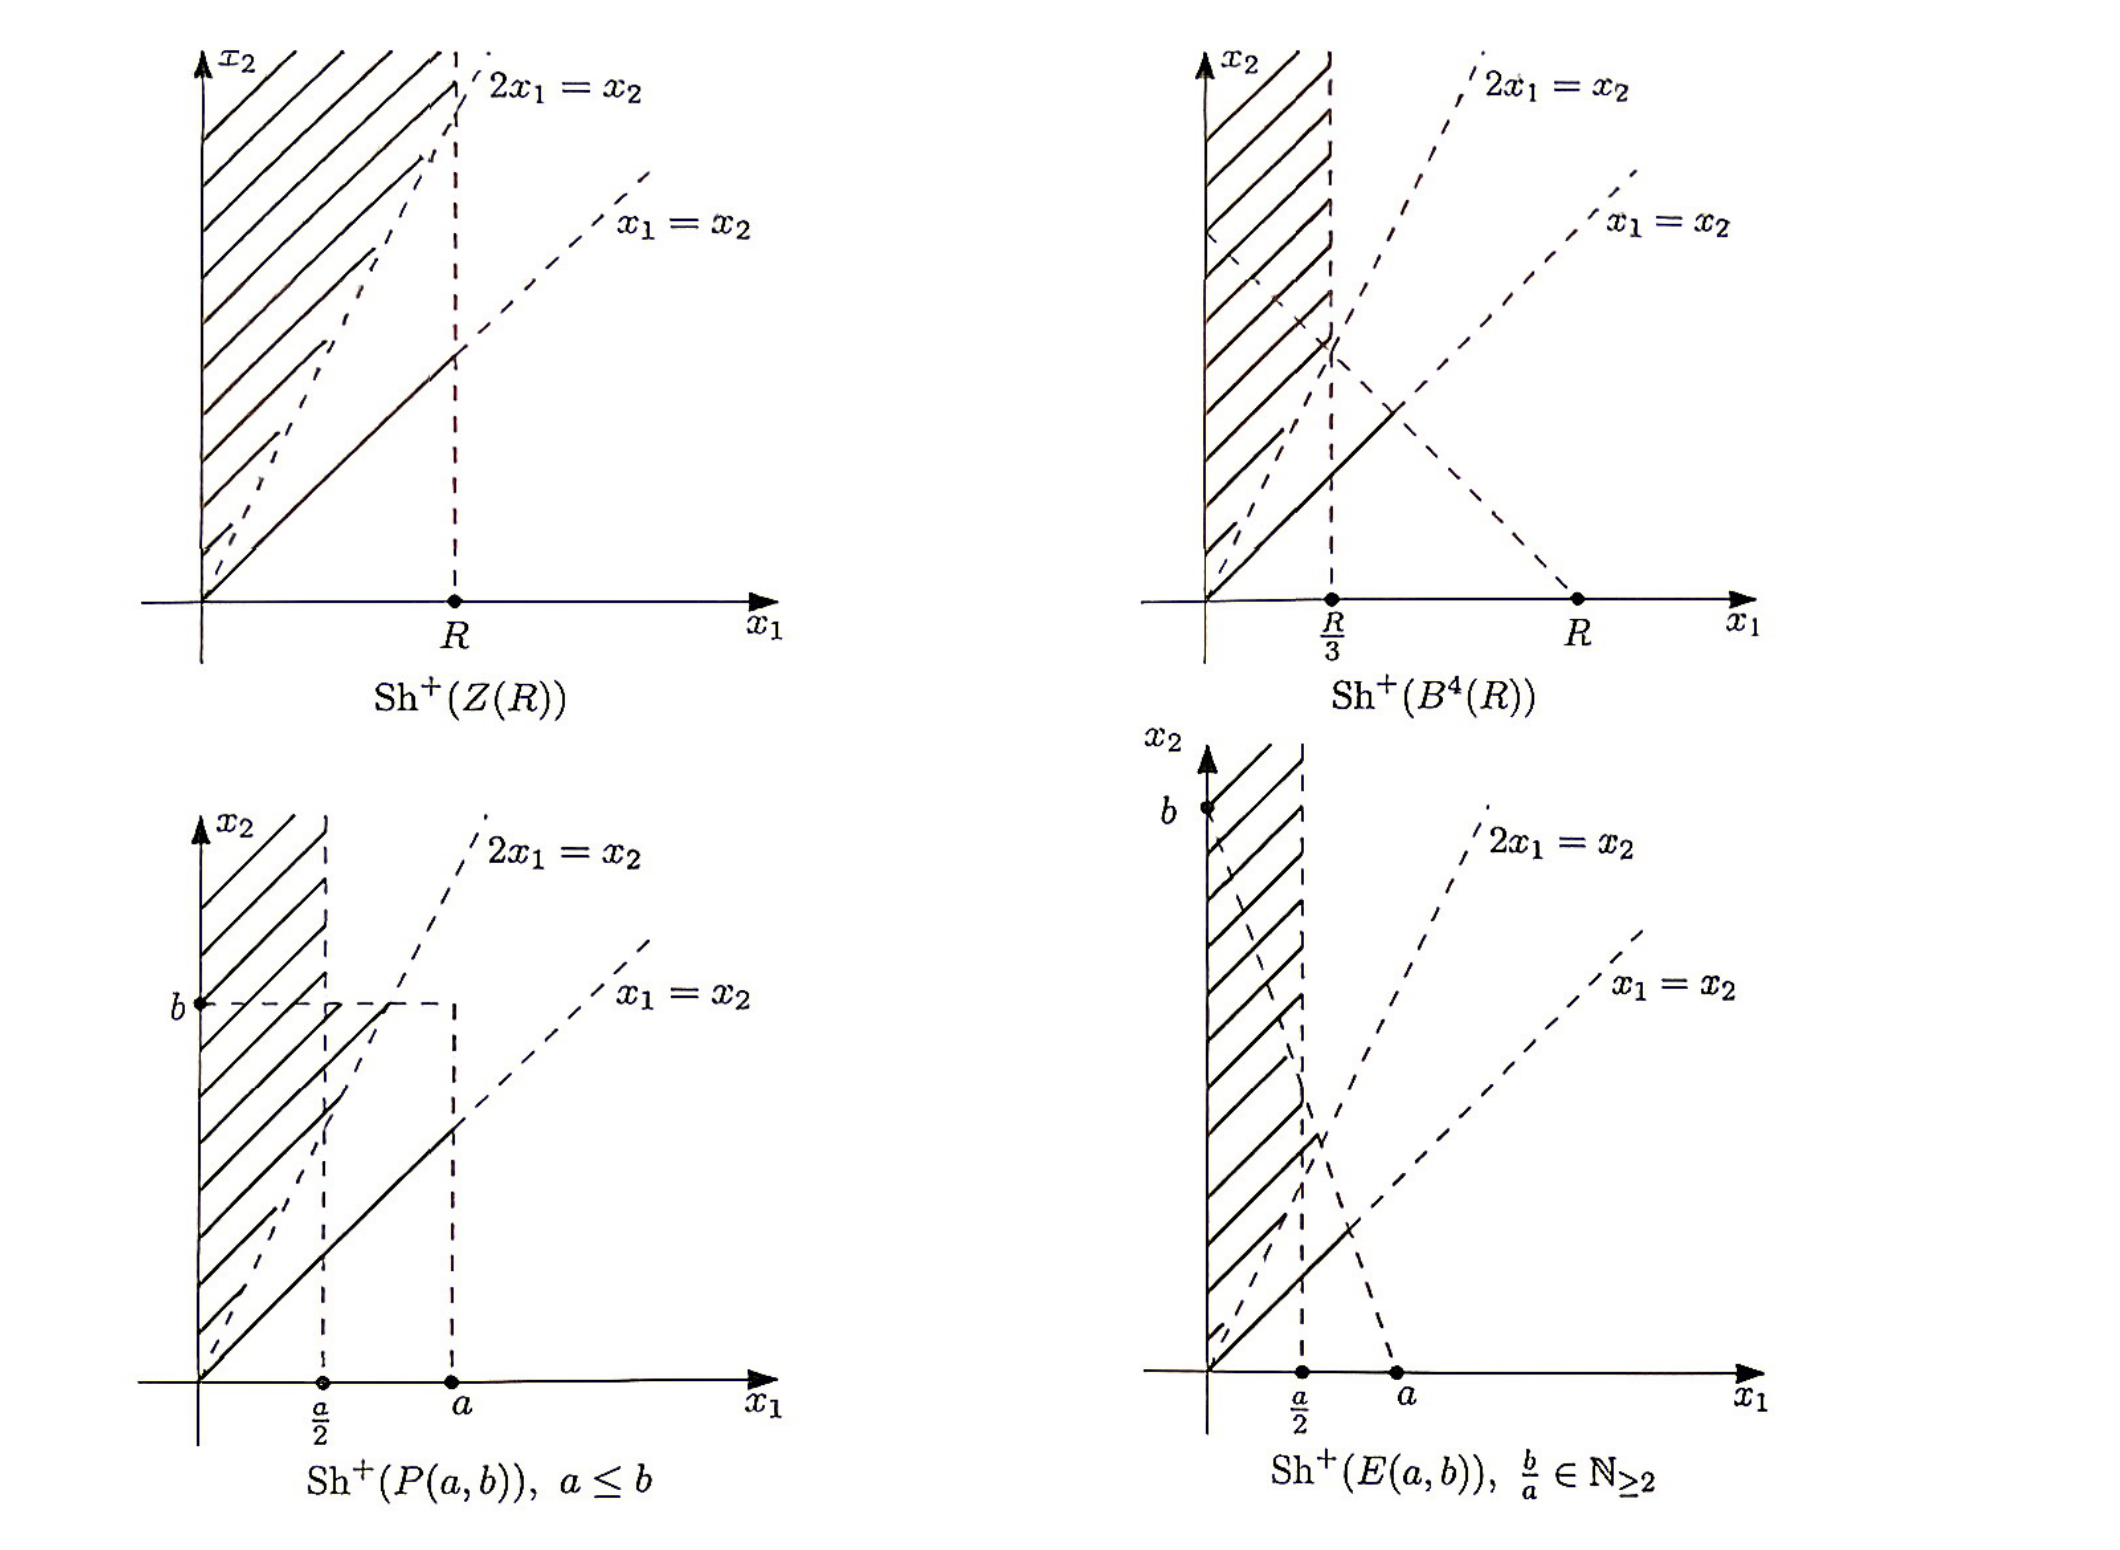
\includegraphics[width=0.92\linewidth]{figures/fig_p201_1.png}
  \caption*{图 7.14\quad 不同基本环面区域 $X_\Omega$ 的
    $\mathrm{Sh}^+(X_\Omega)$ 图像（原书 p.193, Figure 7.14；PDF p.201）}
\end{figure}

\begin{wexam}{7.3.4}
  直接由图 7.14 读出，我们得出
  $\mathrm{Sh}^+(P(1,2))\not\subset\mathrm{Sh}^+(E(1.5,3))$。更精细的图景见
  图 7.15。\hfill$//$
\end{wexam}

\begin{figure}[htbp]
  \centering
  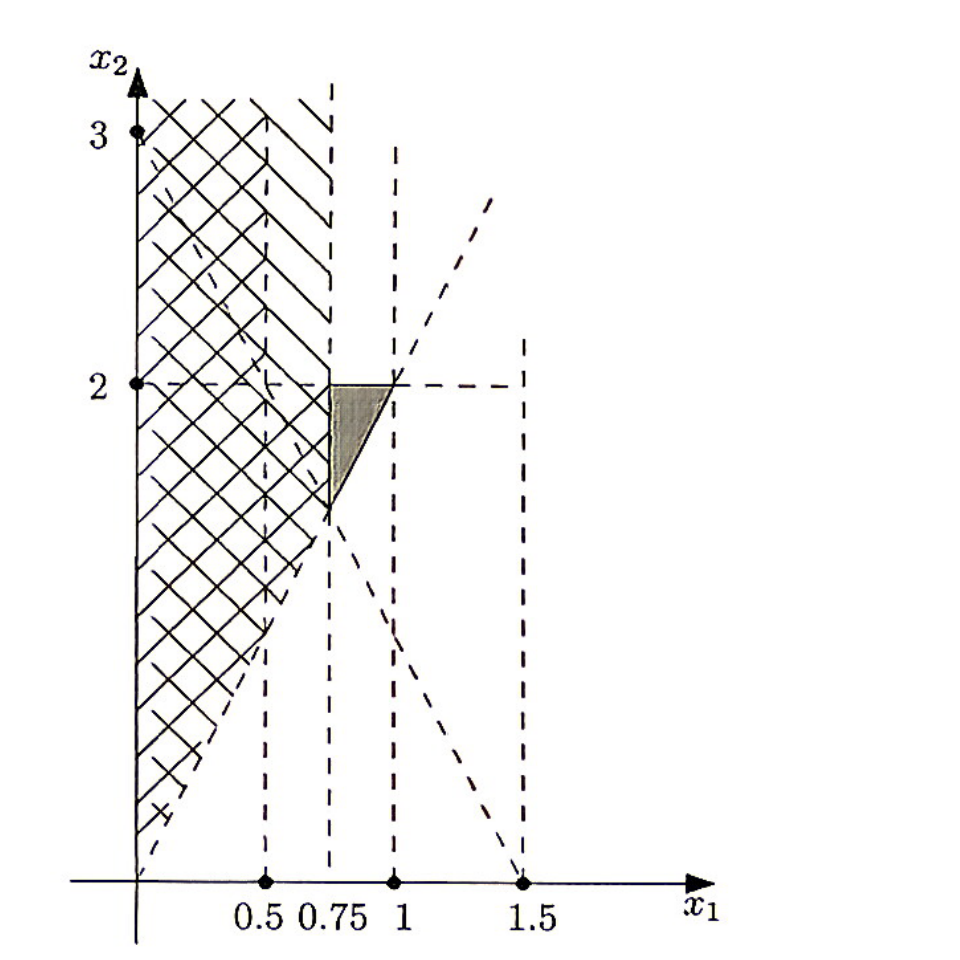
\includegraphics[width=0.52\linewidth]{figures/fig_p201_2.png}
  \caption*{图 7.15\quad 比较 $\mathrm{Sh}^+(P(1,2))$ 与
    $\mathrm{Sh}^+(E(1.5,3))$（原书 p.193, Figure 7.15；PDF p.201）}
\end{figure}

% >>> p202
特别地，灰色部分提供了障碍。所以，$P(1,2)$ 不能辛嵌入 $E(1.5,3)$。注意对
$P(1,2)$ 与 $E(1.5,3)$，体积比较给不出任何障碍（因为
$1\cdot2=2<2.25=(1.5\cdot3)/2$）。此外，Gromov 宽度 $w_G$（(6.24)）也不提供
障碍（因为可以验证 $w_G(P(1,2))=1<1.5=w_G(E(1.5,3))$）。\hfill$//$

\begin{wrem}{7.3.3}
  遗憾的是，形状不变量 $\mathrm{Sh}^+(B^4(R))$ 与 $\mathrm{Sh}^+(Z^4(R))$ 之间
  的直接比较并\emph{不}能重新证出 Gromov 非压缩定理（定理 1.5.1）。这意味着
  仅凭形状不变量 $\mathrm{Sh}^+(\cdot)$，我们无法恢复区域之间辛嵌入的全部信息。
  这大概源于 $\mathrm{Sh}^+(\cdot)$ 的构造——它只基于环面的拉格朗日嵌入。如何
  提取其他子流形的（辛的、定量的）信息，并表述区域的一个辛不变量，是一个值得
  探索的有趣课题。
\end{wrem}
